\chapter{Schlusswort}
Der \textsc{Detroit Electric Car} zeigt sehr gut, dass sich in den letzten einhundert Jahren im grundsätzlichen Bereich der Elektromobilität nicht viel verändert hat: So wird bereits im Oldtimer der Motor über die Spannung und das Feld geregelt, auch wenn heute dazu oftmals ein anderer Motorentyp verwendet wird. In der Schaltung des \textsc{Detroit}s, welche als genial und faszinierend bezeichnet werden muss, wird lediglich beim Anfahren zur ersten Fahrstufe viel Wärme in einem Anfahrwiderstand umgesetzt.

Um möglichst viel im Originalzustand zu belassen, wurde auf grosse Umbauten am Fahrzeug verzichtet. An einigen Stellen war dies jedoch unumgänglich, um so die Funktion und Sicherheit zu gewährleisten. Ebenfalls modifiziert wurden wenn nötig Baugruppen, welche nicht mehr dem Originalzustand entsprachen und somit keinen historischen Wert aufwiesen.

Die verwendete Batterie, welche aus einem verunfallten modernen Elektrofahrzeug stammt, konnte auf das Fahrzeug adaptiert werden. Trotzdem wurden dabei die modernen Funktionen, welche zur Funktions- und Sicherheitsüberwachung von Lithium-Ionen-Zellen nötig sind, berücksichtigt. Für das Fahrzeug resultiert aber, abgesehen vom deutlich kleineren Innenwiderstand der neuen Batterie, kein Unterschied in der Funktionsweise.

Die Arbeiten am \textsc{Detroit} konnten -- bis auf einige Schönheitsfehler -- abgeschlossen werden. Auf Probefahrten hat sich gezeigt, dass die Funktionstüchtigkeit wiederhergestellt werden konnte. Zudem konnten dabei wichtige Erkenntnisse gewonnen werden. Am wichtigsten sei hier sicherlich die Reichweite zu nennen. Hier lagen erste Schätzungen deutlich daneben, beträgt die Reichweite bei realistischer Fahrweise doch nur ungefähr 100 km.

\begin{figure}[h]
	\centering
		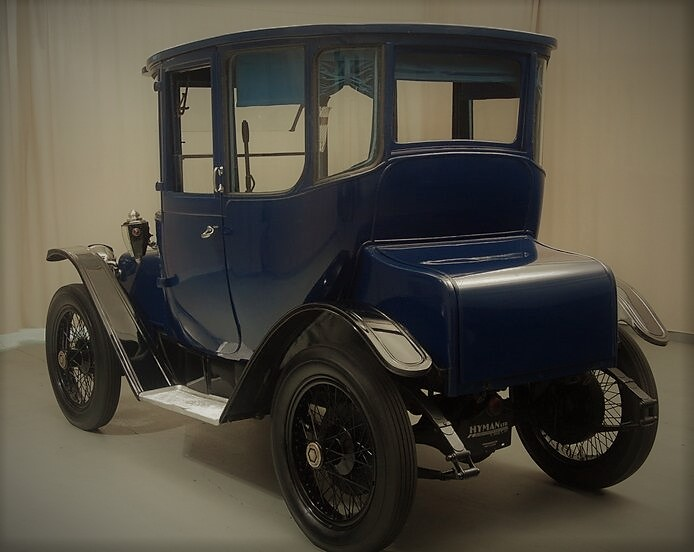
\includegraphics[width=0.75\textwidth]{images/Ende.jpg}
	\label{fig:Ende}
\end{figure}